\chapter{Implementation}

\section{Introduction}

\subsection{Tools}
\subsection{Analysis}
\subsection{Visualizations}
\subsection{Workflow}

\begin{figure}
	\centering
	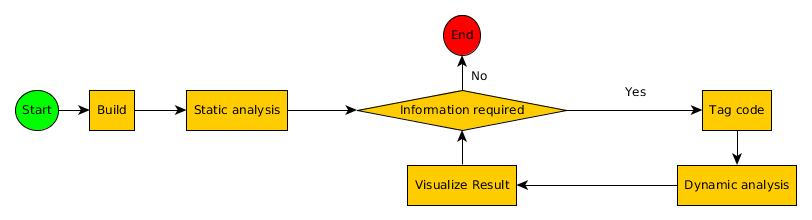
\includegraphics[width=1\textwidth]{workflow}
	\caption{User workflow}
	\label{workflow}
\end{figure}

\subsection{Architecture}

\begin{figure}
	\centering
	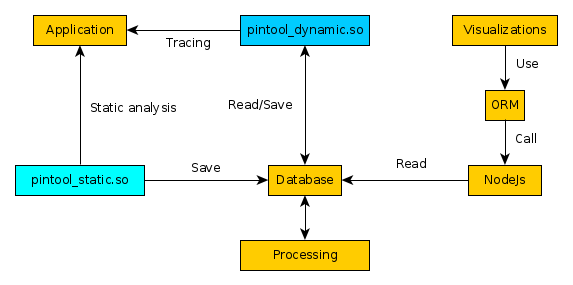
\includegraphics[width=1\textwidth]{architecture}
	\caption{System architecture}
	\label{architecture}
\end{figure}

\section{Concepts}

\subsection{Filtering}

By using dynamic binary instrumentation it is possible to process the entire instruction stream of an application, even dynamic libraries and setup code generated by the compiler. Recording all the actions an application performs might be an advantage, but comes at the cost of runtime overhead and a large tracing database. If a developer is not interested in analyzing the entire application the overhead and the size can be reduced by defining parts that should be ignored.

In Parceive and our implementations three types of filters are available:

\textbf{Image} represents the executable or a shared library and can be used to easily ignore code that is not being developed.

\textbf{Function} represents a routine in the executable. This can be used to filter out modules from inside the executable or shared libraries based on the naming convention of the project.

\textbf{File} allows a developer to filter functions based on the file they were defined in. This requires debug for the component that contains the function. This is also the easiest way to only consider code that has debug information.

\subsection{Tags}

Tags are used to mark interesting parts of the code and to provide input to automatic program analyses. Multiple tag types are available:

\begin{itemize}
	\item [Section] marks the boundaries of a section of code that can be executed in parallel.
	\item [SectionTask] is a task inside a section. Each task can be run in parallel to any other task. When a new task is started, the old one is ended automatically.
	\item [Pipeline] marks the boundaries of a section of code that can be executed in parallel using a pipeline architecture.
	\item [PipelineIteration] represents one iteration of the pipeline.
	\item [PipelineSection] is a section of a iteration. These sections can be run in parallel to different sections from different iterations.
\end{itemize}

\subsubsection{Controling tracing}
Filtering can reduce the amount of data gathered during a programs execution, but tags can provide an even more flexible approach. Using tags it is possible to control tracing during execution with the granularity of a line:

\begin{itemize}
	\item [IgnoreAll] stops all tracing.
	\item [IgnoreCalls] stops the tracing of calls.
	\item [IgnoreAccesses] stops the tracing of accesses.
	\item [ProcessAll] forces the tracing of everything.
	\item [ProcessCalls] forces the tracing of calls.
	\item [ProcessAccesses] starts the tracing of accesses.
\end{itemize}

In Figure \ref{cap3:contralg} we can see the algorithm used to determine whether tracing is performed.

\begin{figure}
	\begin{center}
		\begin{minted}{c}
			if (ignoreCalls)
				processCallsComputed = false;
			else if (processCalls)
				processCallsComputed = true;
			else if (interestingProgramPart)
				processCallsComputed = true;
			else
				processCallsComputed = true;
			
			if (!processCallsComputed)
				processAccessesComputed = false;
			else if (ignoreAccesses)
				processAccessesComputed = false;
			else if (processAccesses)
				processAccessesComputed = true;
			else if (interestingProgramPart)
				processAccessesComputed = true;
			else
				processAccessesComputed = false;
		\end{minted}
	\end{center}
	\caption{Algorithm to determine if tracing is performed}
	\label{cap3:contralg}
\end{figure}

\subsection{Tools}

As part of this thesis two tools have been developed: \texttt{pintool\_static.so} and \texttt{pintool\_dynamic.so}.

\subsection{Analysis}

\texttt{pintool\_dynamic.so} and the database processing analyze the information gathered during the tracing in order to provide insight into the program. 

\subsection{Visualizations}

Additional visualizations have been implemented to enable source code tagging and to display the information obtained by the analysis:

\textbf{File View}

\textbf{Tag List}

\textbf{Section View}

\textbf{Pipeline View}

Additionally existing views have been extended to provide more information about tags:

\textbf{Detail View}

\textbf{CCT View}

\subsection{Database layout}

Additional tables have been added to the parceive database to store information about tags and the layout of the source code. The \texttt{SourceLocation} table contains all locations in the code that are referenced in the debug information and can be used for tags.

\subsection{pintool\_static.so}

\texttt{pintool\_static.so} performs static analysis on the executable and all the loaded dynamic libraries to determine the relationship between the source code and the executable. The instrumented application is executed to discover the dynamic libraries loaded at runtime.

\subsubsection{Source Locations}

Performing the analysis generates a database of all locations where a tag can be inserted into the application source code. This information is important because it is not obvious which line of code results in executable instructions, especially at block boundaries.

\subsubsection{File View}

The File View can render the files that were used to build the instrumented application.

\subsubsection{Tagging}

The File View can tag sections of the source code to generate an input for the dynamic analysis. 

\subsection{pintool\_dynamic.so}

\texttt{pintool\_static.so} performs a dynamic analysis on the application.

\subsubsection{Architecture}



\subsubsection{Fast buffer API}
\subsubsection{Allocation interception}
\subsubsection{Shadow Stack}
\subsubsection{Tagging implementation}
\subsubsection{Memory accesses}
\subsubsection{Reference resolution}
\subsubsection{Thread handling}
\subsubsection{Tag handling}

\section{Analysis}

\subsection{Section}
\subsubsection{Introduction}
\subsubsection{Parallelization}
\subsubsection{Dependency detection}
\subsubsection{Visualization}

\subsection{Pipeline}
\subsubsection{Introduction}
\subsubsection{Parallelization}
\subsubsection{Dependency detection}
\subsubsection{Visualization}

\subsection{Calling Context Tree}
\subsubsection{Parceive UI}
\subsubsection{Modifications}





